\section*{Lezione 17}
\addcontentsline{toc}{section}{Lezione 17}

\subsection*{AES}
\addcontentsline{toc}{subsection}{AES}

La competizione degli anni '90 viene vinta da Rijndael e il suo AES, esso diventa standard dal 2002. Cifra blocchi di 128 bit per volta e le chiavi possono essere di diverse lunghezze (AES-128, AES-192 e AES-256). \'E più efficiente di DES e la sua implementazione software è più semplice.
Per semplicità vediamo solo AES-128, ma gli altri cambiano solo su pochi dettagli.
\begin{itemize}
	\item \textbf{Cifratura}: l'algoritmo opera su una matrice di stato 4x4 di 16 bytes (128 bits). Inizialmente la matrice contiene il blocco del messaggio in chiaro (riempita per colonne).\\
	Vengono generate le chiavi derivate e si effettua uno XOR fra i bit della matrice e quelli della \textbf{Roundkey}.
	Per nove volte (ogni chiave derivata) si effettuano queste operazioni:
		\begin{enumerate}
			\item \textbf{SubBytes} (sostituzione dei byte utilizzando una S-box)\\
			Essa è una operazione invertibile ma non lineare. Si fissa $b=(b_7,b_6,...,b_0)$ e si definiscono:
			\begin{figure}[h]
				\centering
				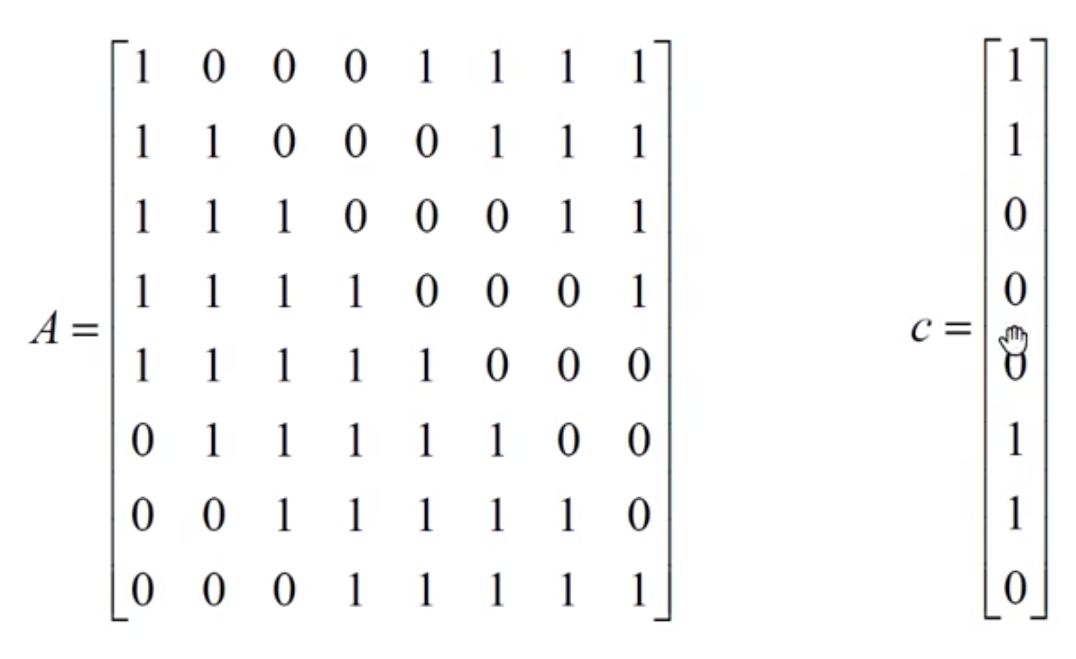
\includegraphics[width=0.7\linewidth]{immagini/img35}
			\end{figure}
			Poi, se $b\neq 0$ allora $b=b^{-1}$ e si ritorna $A \cdot b + c$.\\
			La non linearità sta nel calcolo dell'inverso di $b$ (resistenza ad attacchi ad approssimazione). Vedo i termini di $b$ come i coefficienti di un equazione di settimo grado ($b_7x^7 + b_6x^6 + \dots + +b_1x + b_0$), poi faccio la divisione con resto con il polinomio irriducibile $x^8+x^4+x^3+x+1$ nel campo $GF(2^8)$ ovvero con resto 0 o 1. In questo campo ci sono vettori di 8 elementi, la somma è lo xor, il prodotto poi si divide per lo stesso vettore.
			
			
			
			
			\item \textbf{Shiftrows} (rotazione delle righe)\\
			La prima riga rimane alterata, la seconda la terza e la quarta viene ruotata di 1, 2, 3 posizioni rispettivamente
			
			\item \textbf{MixColumns} (operazioni sulle colonne)\\
			Moltiplica ogni colonna per una matrice fissata e che diventa la nuova colonna.
			
			\item \textbf{AddRoundKey} (come prima, si effettua uno xor)
		\end{enumerate} 
		
	Come si generano le chiavi derivate? Spieghiamo per AES-128.
	Bisogna ottenere 11 chiavi, ognuna di 16 bytes. L'algoritmo lavora su parole di 4 byter, quindi dobbiamo ottenere 44 parole che inseriamo in un array $w[0,..43]$. Si definiscono 10 costanti $Rcon[1]$, $Rcon[2]$, ..., $Rcon[10]$. Successivamente si segue questo pseudocodice:
	
		\begin{figure}[h]
		\centering
		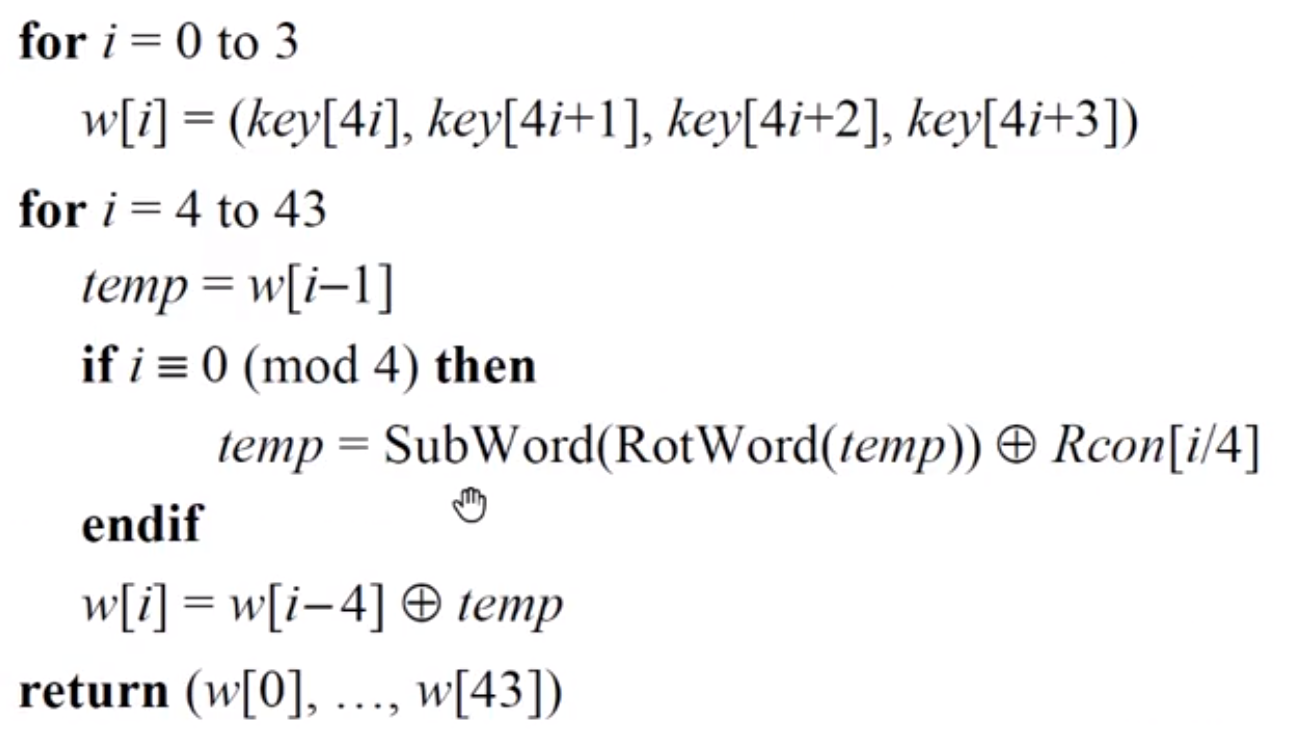
\includegraphics[width=0.9\linewidth]{immagini/img36}
	\end{figure}

\subsection*{Crittosistemi simmetrici}
\addcontentsline{toc}{subsection}{Crittosistemi simmetrici}

Abbiamo una sequenza di testi di in chiaro $m_1, m_2, ...$ di testi in chiaro e una chiave iniziale $k$, vogliamo avere una sequenza di testi cifrati $c_1, c_2,...$.\\
\textbf{Modi di operazione}: 
\begin{itemize}
	\item ECB (Electronic CodeBook)\\
	Il più semplice, ma anche il meno sicuro: ho $m_1$, lo cifro usando $E_k$ e ottengo $c_1$ (e così via per tutte le $m$). Quando Eve comincia ad ascoltare (mettiamo che si perda alcuni pezzi), non ha vita difficile visto che ogni operazione di cifratura è indipendente dalla precedente. Oppure esempio pinguino Linux, cifro blocchi uguali in modo uguale, il risultato sarà strano ma avrà la forma del pinguino (il pattern non viene rotto).
\end{itemize}


	
\end{itemize}
